\documentclass[12pt,a4paper]{report}
\usepackage[utf8]{inputenc}
\usepackage[french]{babel}
\usepackage{tikz}
\usepackage{listings}
\usepackage{amsmath}
\usepackage{amsfonts}
\usepackage[T1]{fontenc}
\usepackage{amssymb}
\usepackage{graphicx}
\usepackage{color} 
\usepackage{fancybox}
\usepackage{biblatex}
\usepackage{lmodern}
\usepackage{tikz}
\usepackage{relsize}
\usepackage{float}
\usepackage{caption}
\usepackage{subcaption}
\usepackage{arabtex}
\usepackage{utf8}
\usepackage{pgfplots}
\usepackage{algorithmicx}
\usepackage{algpseudocode}
\usepackage{wrapfig}
\usepackage{tikz}
\usepackage{listings}
\usepackage{xcolor}
\usetikzlibrary{shadows}
\algdef{SE}[DOWHILE]{Do}{doWhile}{\algorithmicdo}[1]{\algorithmicwhile\ #1}%
\usepackage{comment}
\usepackage{lipsum}
\usepackage[ruled,vlined, french, onelanguage]{algorithm2e}
\usepackage{fancyhdr}
\usepackage{hyperref}
\usepackage{fancybox}
\usepackage[left=3cm, right=3cm, top=3.00cm, bottom=3.5cm]{geometry}
\usepackage{mdframed}
\usepackage[Glenn]{fncychap}
\graphicspath{{./figures/}}
\renewcommand{\baselinestretch}{1.2}
\graphicspath{{figures/}}
% Configuration du style du code
\lstset{
    language=Python, % Langage du code
    basicstyle=\small\ttfamily, % Style de base
    keywordstyle=\color{blue}, % Couleur des mots-clés
    commentstyle=\color{green!40!black}, % Couleur des commentaires
    stringstyle=\color{orange}, % Couleur des chaînes de caractères
    breaklines=true, % Activation du retour à la ligne automatique
    numbers=left, % Affichage des numéros de ligne
    numberstyle=\tiny\color{gray}, % Style des numéros de ligne
    stepnumber=1, % Intervalle entre deux numéros de ligne
    showstringspaces=false, % Ne pas afficher les espaces dans les chaînes de caractères
    frame=single, % Affichage d'un cadre autour du code
    backgroundcolor=\color{gray!10}, % Couleur de fond
    captionpos=b % Position de la légende
}
\begin{document}
\begin{center}
\thispagestyle{empty}
\rule{1\textwidth}{0,5pt}\vspace{0,5cm}\\
\textbf{Université de montpellier\\
Faculté des sciences}\\
\vspace{1cm}
\includegraphics[width=4cm, height=4cm]{MONTPELLIER.jpg}
\end{center}

\begin{center}
\textbf{Département mathématique}
\vspace{1cm}
\hspace{2cm}\\
\textbf{\huge{TP 3}} \\
\vspace{1cm}
\textbf{M2 MIND-SIAD}
\vspace{1cm}

\rule{0,9\textwidth}{3pt}\\
\vspace{0,3cm}
\large\textit{\textbf{ Support Vector Machine (SVM)}}
\normalsize
\rule{0,9\textwidth}{3pt}\\ 
 
\end{center}
\vspace{1cm}
\hspace{0,2cm}
\begin{center}
\textbf{Réalisé par :}
\hspace*{0,3cm}HAMOMI Majda
\end{center}



\\
\vspace{1cm}
\begin{center}
\textbf{Septembre 2024 }
\end{center}
\pagestyle{plain}




\tableofcontents
\newpage

\section*{Introduction  }
\addcontentsline{toc}{chapter}{Introduction }
Les machines à vecteurs de support (SVM) sont des techniques de classification supervisée, particulièrement populaires pour leur capacité à gérer des problèmes de classification binaire en séparant les données à l'aide d'hyperplans optimaux. Ce TP vise à implémenter et évaluer des modèles SVM à travers plusieurs scénarios, en explorant différents noyaux, l'impact des paramètres de régularisation, l'ajout de variables de nuisance, et l'amélioration des performances avec la réduction de dimension via PCA.
\section{Généralités et Fondements Mathématiques des SVM}

\subsection{Introduction aux SVM}

Les \textit{Support Vector Machines} (SVM), introduits par Vladimir Vapnik dans les années 90, sont utilisés pour résoudre des problèmes de classification binaire. Leur principe repose sur la recherche d'un hyperplan affine qui sépare au mieux les données appartenant à deux classes distinctes, tout en maximisant la marge de séparation entre elles. Cet hyperplan est défini comme celui qui maximise la distance minimale entre les points des deux classes, appelés vecteurs de support.

\subsection{Classification binaire supervisée}

Soit un jeu de données constitué d'observations \( x = (x_1, ..., x_p) \in X \subset \mathbb{R}^p \) avec des étiquettes \( y \in \{−1, 1\} \). Dans le cadre de la classification binaire, le problème consiste à trouver une fonction \( \hat{f} : X \to \{-1, 1\} \) qui prédit l'étiquette d'une nouvelle observation en fonction de sa position par rapport à un hyperplan séparateur.

L'hyperplan affine est défini par l'équation \( \langle w, x \rangle + w_0 = 0 \), où \( w \in \mathbb{R}^p \) est un vecteur normal à l'hyperplan et \( w_0 \) est le biais. La règle de décision est donc la suivante :
\[
\hat{f}(x) = \text{sign}\left(\langle w, x \rangle + w_0\right).
\]
Ainsi, selon que \( \hat{f}(x) \) est positif ou négatif, l'étiquette prédite sera \( +1 \) ou \( -1 \).

\subsection{SVM et espace de grande dimension}

Dans le cas où les données ne sont pas linéairement séparables dans leur espace d'origine \( X \), les SVM utilisent une fonction de transformation non linéaire \( \Phi \) qui projette les données dans un espace de plus grande dimension, appelé espace de caractéristiques (ou espace de Hilbert \( H \)). L'objectif est de rendre les données linéairement séparables dans cet espace transformé.

Cependant, il est souvent coûteux de calculer explicitement cette transformation. Pour contourner cela, les SVM utilisent l'astuce du noyau (\textit{kernel trick}), qui permet de calculer directement les produits scalaires dans l'espace transformé sans avoir à effectuer explicitement la transformation :
\[
K(x, x') = \langle \Phi(x), \Phi(x') \rangle.
\]
Quelques noyaux classiques incluent :
\begin{itemize}
    \item \textbf{Noyau linéaire} : \( K(x, x') = \langle x, x' \rangle \),
    \item \textbf{Noyau gaussien RBF} : \( K(x, x') = \exp(-\gamma \| x - x' \|^2) \),
    \item \textbf{Noyau polynomial} : \( K(x, x') = (\alpha \langle x, x' \rangle + \beta)^\delta \).
\end{itemize}

\subsection{Problème d'optimisation}

Le classifieur SVM cherche à maximiser la marge entre les classes tout en minimisant l'erreur de classification. Ce problème est formulé comme suit :
\[
\min_{w, w_0, \xi} \left( \frac{1}{2} \| w \|^2 + C \sum_{i=1}^n \xi_i \right),
\]
sous les contraintes \( \xi_i \geq 0 \) et \( y_i (\langle w, \Phi(x_i) \rangle + w_0) \geq 1 - \xi_i \) pour tout \( i \).

La solution optimale peut être exprimée en fonction des vecteurs de support \( x_i \), c’est-à-dire les points de données pour lesquels les contraintes sont actives ( \( \alpha_i \neq 0 \) dans la formulation duale). Les vecteurs \( w \) et \( w_0 \) sont ajustés en résolvant un problème d'optimisation quadratique sous contraintes affines.

\subsection{Contrôle de la complexité et régularisation}

Le paramètre \( C \) joue un rôle clé dans le contrôle de la complexité du modèle. Un \( C \) élevé force le modèle à minimiser les erreurs de classification, au risque de surapprendre, tandis qu'un \( C \) faible favorise une meilleure généralisation en tolérant quelques erreurs de classification.

Une alternative au réglage direct de \( C \) est la méthode de \(\nu\)-classification, qui permet de contrôler la fraction de vecteurs de support parmi les données d'apprentissage via un paramètre \( \nu \in [0, 1] \).

\subsection{Extensions au cas multi-classes}

Pour traiter des problèmes de classification multi-classes ( \( Y \in \{1, ..., K\} \)), les approches les plus courantes sont :
\begin{itemize}
    \item \textbf{Un contre un} : Construire un classifieur pour chaque paire de classes ( \( K(K-1)/2 \) classifieurs en tout),
    \item \textbf{Un contre tous} : Construire un classifieur pour chaque classe \( k \), en séparant les données où \( Y = k \) des autres classes.
\end{itemize}


\section{SVM sur le Dataset Iris}

Dans cette première partie, nous avons utilisé la bibliothèque \texttt{scikit-learn} pour implémenter les \textit{Support Vector Machines} (SVM). Le dataset \texttt{Iris} contient trois classes de fleurs : Setosa, Versicolor et Virginica. Nous avons restreint cette étude à une classification binaire, en ne considérant que les deux premières classes (Setosa et Versicolor) et les deux premières variables. Le but est de comparer la performance d’un SVM avec noyau linéaire et un SVM avec noyau polynomial.

\subsection{Chargement des données et prétraitement}

Nous avons commencé par charger le jeu de données Iris et appliqué une normalisation pour centrer et réduire les données, à l'aide de la classe \texttt{StandardScaler}. Ensuite, nous avons filtré les observations pour ne garder que les deux premières classes et les deux premières variables. Une division des données en ensembles d'entraînement (50 \%) et de test (50 \%) a été effectuée pour évaluer les modèles.

\begin{lstlisting}[language=Python, caption=importation des packages]
from sklearn import datasets
from sklearn.preprocessing import StandardScaler
from sklearn.model_selection import train_test_split, GridSearchCV
from sklearn.utils import shuffle
import numpy as np
\end{lstlisting}
\begin{lstlisting}[language=Python, caption=Chargement des données et prétraitement]
# Charger les données Iris
iris = datasets.load_iris()
X = iris.data
scaler = StandardScaler()  # Normalisation des données
X = scaler.fit_transform(X)
y = iris.target
# Filtrer pour garder uniquement les classes 1 et 2 et les deux premières variables
X = X[y != 0, :2]
y = y[y != 0]
# Diviser les données en ensemble d'entraînement et de test
X, y = shuffle(X, y, random_state=42)
X_train, X_test, y_train, y_test = train_test_split(X, y, test_size=0.5, random_state=42)
\end{lstlisting}
\subsection{Classification de la Classe 1 contre la Classe 2 du Dataset Iris avec un Noyau Linéaire}
\paragraph{SVM avec noyau linéaire\\}
Dans un premier temps, nous avons implémenté un SVM avec un noyau linéaire. Pour trouver le meilleur paramètre de régularisation \( C \), nous avons utilisé une recherche par grille (\texttt{GridSearchCV}), en testant différentes valeurs de \( C \) sur une échelle logarithmique.



\begin{lstlisting}[language=Python, caption=Implémentation du SVM avec noyau linéaire]
# Définir la grille de paramètres pour le noyau linéaire
parameters = {'kernel': ['linear'], 'C': list(np.logspace(-3, 3, 200))}
# Utiliser GridSearchCV pour trouver les meilleurs paramètres
clf_linear = GridSearchCV(SVC(), parameters, cv=5)
clf_linear.fit(X_train, y_train)
# Afficher le meilleur paramètre C et la précision
print('Meilleur paramètre C pour le noyau linéaire :', clf_linear.best_params_)
print('Generalization score for linear kernel: %s, %s' %
      (clf_linear.score(X_train, y_train),
       clf_linear.score(X_test, y_test)))
\end{lstlisting}

\textbf{Résultats} : Le meilleur paramètre \( C \) trouvé est de \textbf{0.2967}, Le modèle avec un noyau linéaire obtient une précision de \textbf{66 \%} à la fois sur les données d'entraînement et sur les données de test. Cela indique que le modèle est bien régularisé et qu'il ne présente pas de sur-apprentissage ni de sous-apprentissage, mais que la séparation linéaire n'est pas parfaite pour ces données. 
\subsection{Comparaison des Performances entre un Noyau Linéaire et un Noyau Polynomial}
\paragraph{SVM avec noyau polynomial\\}
Ensuite, nous avons utilisé un SVM avec un noyau polynomial pour capturer des relations non linéaires potentielles dans les données. Nous avons testé différentes valeurs du degré du polynôme, ainsi que du paramètre \( C \) et \( \gamma \).



\begin{lstlisting}[language=Python, caption=Implémentation du SVM avec noyau polynomial]
# Définir la grille de paramètres pour le noyau polynomial
Cs = list(np.logspace(-3, 3, 5))
gammas = 10. ** np.arange(1, 2)
degrees = np.r_[2, 3]
parameters = {'kernel': ['poly'], 'C': Cs, 'gamma': gammas, 'degree': degrees}
# Utiliser GridSearchCV pour le noyau polynomial
clf_poly = GridSearchCV(SVC(), parameters, cv=5)
clf_poly.fit(X_train, y_train)
# Afficher les meilleurs paramètres et la précision
print(clf_poly.best_params_)
print('Generalization score for polynomial kernel: %s, %s' %
      (clf_poly.score(X_train, y_train),
       clf_poly.score(X_test, y_test)))
\end{lstlisting}
\textbf{Résultats} : \\
Meilleurs paramètres pour le noyau polynomial
\begin{itemize}
    \item \textbf{\( C = 0.0316 \)} : Ce paramètre de régularisation est assez petit, ce qui suggère que le modèle tolère plus d'erreurs dans les données d'entraînement pour éviter de sur-apprendre. Le faible \( C \) permet au modèle de généraliser davantage, mais il risque aussi de sous-apprendre si les données sont bien séparées.
    
    \item \textbf{\( \text{degree} = 1 \)} : Le degré du noyau polynomial est de 1, ce qui signifie qu'en réalité, il se comporte comme un noyau linéaire. Cela suggère que le noyau polynomial n'a pas trouvé de relations non linéaires significatives dans les données.
    
    \item \textbf{\( \gamma = 10.0 \)} : Le paramètre \( \gamma \) contrôle l'influence d'un seul point d'entraînement. Un \( \gamma \) élevé (comme ici, 10.0) indique que le modèle considère les points proches de la frontière de décision de manière plus importante, ce qui peut potentiellement créer des frontières plus complexes.
\end{itemize}
Les scores de généralisation montrent que le modèle polynomial obtient une précision de 66 \% sur l'ensemble d'entraînement, indiquant qu'il n'a pas sur-appris. La précision est identique sur l'ensemble de test, suggérant une généralisation cohérente, mais modérée. Cela indique que la complexité du noyau polynomial n'apporte pas d'amélioration par rapport à un modèle linéaire.

\paragraph{Visualisation des résultats\\}

Enfin, nous avons visualisé les frontières de décision générées par les deux modèles (noyau linéaire et noyau polynomial). Les figures ci-dessous montrent les données projetées dans l’espace bidimensionnel ainsi que les frontières séparatrices.

\begin{lstlisting}[language=Python, caption=Visualisation des résultats]
def f_linear(xx):
    """Classifier: needed to avoid warning due to shape issues"""
    return clf_linear.predict(xx.reshape(1, -1))
def f_poly(xx):
    """Classifier: needed to avoid warning due to shape issues"""
    return clf_poly.predict(xx.reshape(1, -1))
def plot_2d(X, y):
    plt.scatter(X[:, 0], X[:, 1], c=y, cmap='autumn')
    plt.xlabel('Feature 1')
    plt.ylabel('Feature 2')
def frontiere(f, X, y, step=50):
    x_min, x_max = X[:, 0].min() - 1, X[:, 0].max() + 1
    y_min, y_max = X[:, 1].min() - 1, X[:, 1].max() + 1
    xx, yy = np.meshgrid(np.linspace(x_min, x_max, step), np.linspace(y_min, y_max, step))
    Z = np.array([f(np.array([xx_, yy_])) for xx_, yy_ in zip(xx.ravel(), yy.ravel())])
    Z = Z.reshape(xx.shape)
    plt.contourf(xx, yy, Z, alpha=0.8, cmap='autumn')
    plt.scatter(X[:, 0], X[:, 1], c=y, edgecolor='k', s=20)
plt.ion()
plt.figure(figsize=(15, 5))
plt.subplot(131)
plot_2d(X, y)
plt.title("iris dataset")
plt.subplot(132)
frontiere(f_linear, X, y)
plt.title("linear kernel")
plt.subplot(133)
frontiere(f_poly, X, y)
plt.title("polynomial kernel")
plt.tight_layout()
plt.show()
\end{lstlisting}
\begin{figure}[H]
    \centering
    \begin{minipage}{0.9\textwidth}
        \centering
        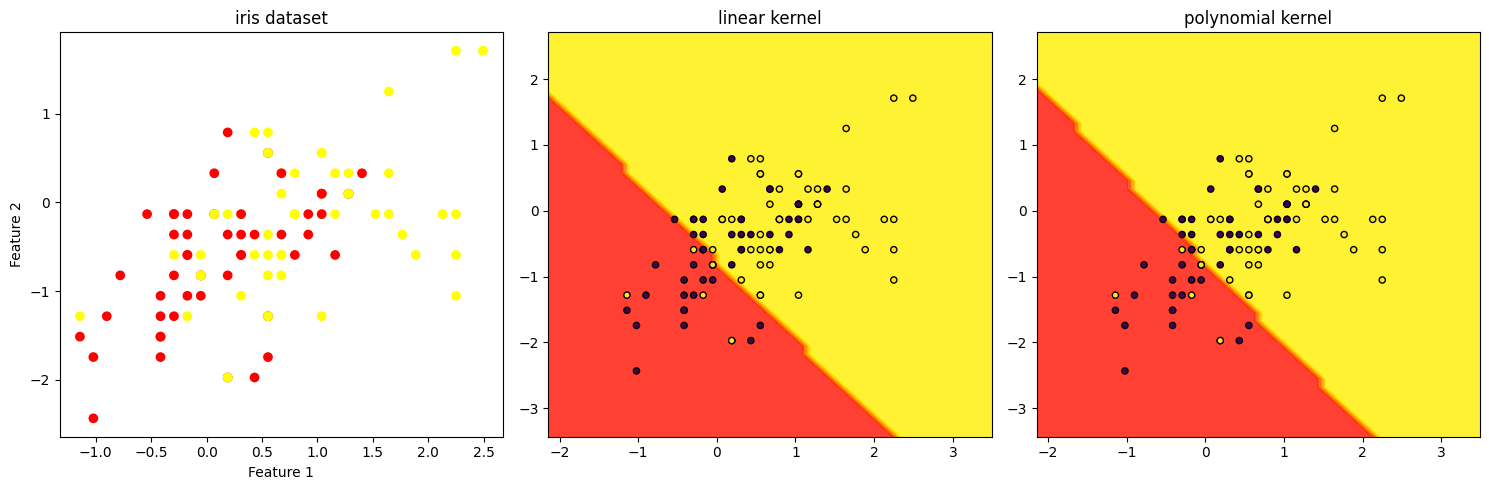
\includegraphics[width=\textwidth]{output.png}
        \caption{ Classifications avec noyaux linéaire et polynomial (degré 1) }
    \end{minipage}
    \end{figure}
 

La Figure 1 présente la classification des données du dataset Iris à l’aide d’un noyau linéaire avec des paramètres optimaux \(\{C : 0.031, \text{degree} : 1, \gamma : 10.0, \text{kernel} : \text{poly}\}\). Le modèle linéaire génère des frontières de décision bien définies, permettant une séparation efficace des classes. Les scores de généralisation, à \(0.66\) pour l’entraînement et le test, montrent que le modèle capture bien les tendances des données sans surajuster ou sous-ajuster. Un paramètre de régularisation \(C\) légèrement plus élevé favorise une bonne adaptation aux données d’entraînement tout en maintenant une capacité de généralisation solide. En conclusion, la Figure 1 illustre qu’un modèle linéaire est approprié et efficace pour cette tâche.


   
\begin{figure}[H]
    \centering
    \begin{minipage}{0.9\textwidth}
        \centering
        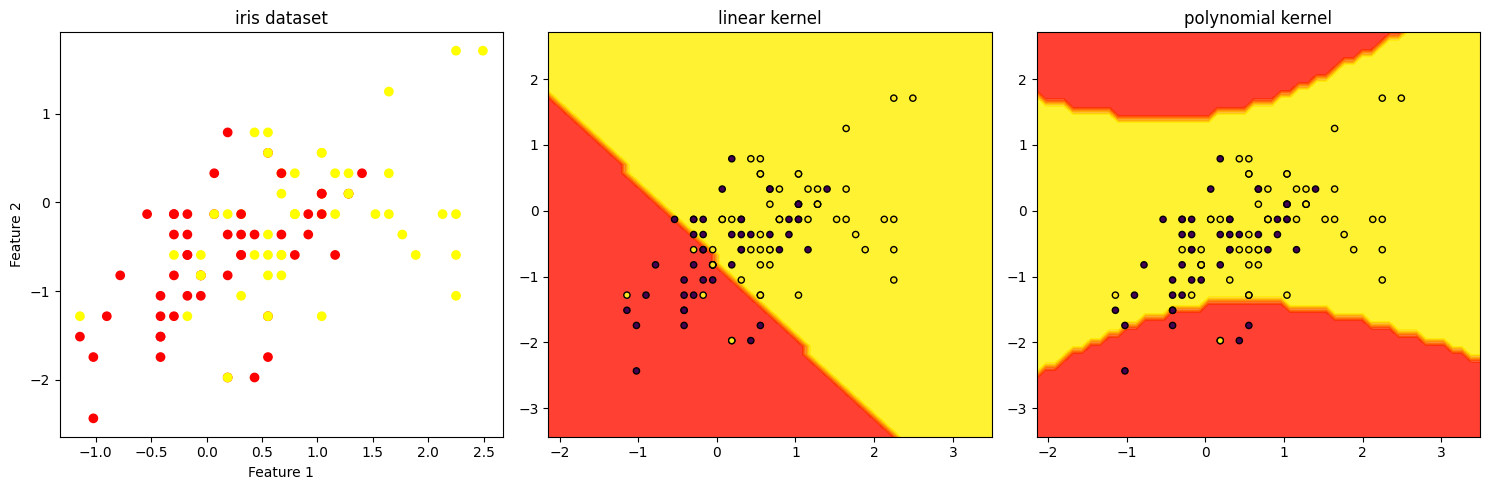
\includegraphics[width=\textwidth]{output1.png}
        \caption{ Classifications avec noyaux linéaire et polynomial (degré 2) }
    \end{minipage}
    \end{figure}  

En revanche, la Figure 2 met en évidence l'effet d'une séparation quadratique des données avec un noyau polynomial de degré 2, utilisant les paramètres optimaux $\{C: 0.001, \text{degree}: 2, \gamma: 10.0, \text{kernel}: \text{poly}\}$. Bien que ce modèle soit capable de modéliser des frontières de décision plus complexes, il souffre d'une performance inférieure, comme en témoignent les scores de généralisation : $0.64$ sur l'entraînement et $0.44$ sur le test. Un faible paramètre $C$, égal à $0.001$, indique que le modèle privilégie une grande marge de séparation, entraînant ainsi un \textit{underfitting} où il ne capture pas suffisamment d'informations à partir des données d'entraînement. Cela se traduit par une difficulté à généraliser sur de nouvelles données, suggérant que la régularisation est trop forte.

\section{Impact du Noyau Linéaire et du Paramètre C sur un Jeu Déséquilibré}

Dans cette section, nous avons exécuté le fichier \texttt{svm\_gui.py} tout en générant un jeu de données très déséquilibré, avec une distribution de points où une classe représente au moins 90\% des données et l'autre seulement 10\%. En ajustant le paramètre de régularisation \( C \) dans un SVM avec noyau linéaire, nous avons obtenu les graphes suivants, illustrant l'impact de \( C \) sur la séparation des classes.


\begin{figure}[H]
    \centering
    \begin{minipage}{0.5\textwidth}
        \centering
        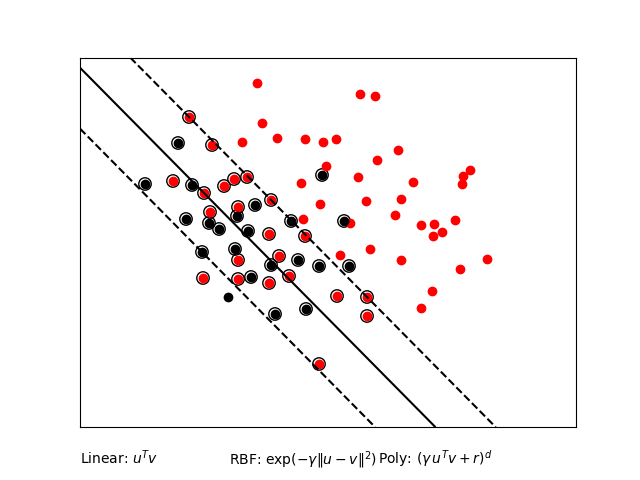
\includegraphics[width=\textwidth]{im1.png}
        \caption{SVM avec C = 1}
    \end{minipage}\hfill
    \begin{minipage}{0.5\textwidth}
        \centering
        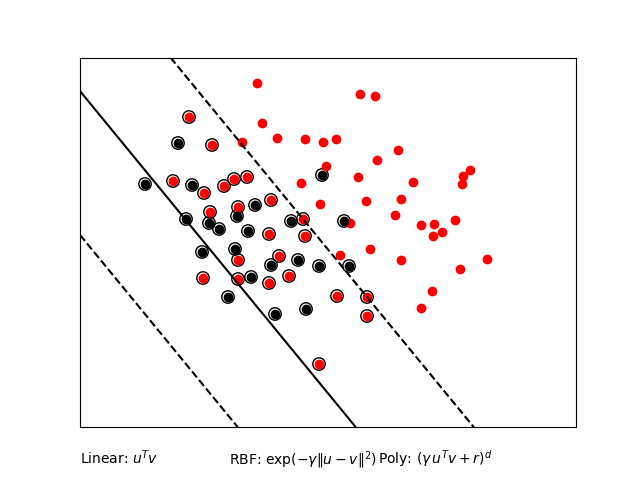
\includegraphics[width=\textwidth]{IM00019.png}
        \caption{SVM avec C = 0.0019}
    \end{minipage}
    \begin{minipage}{0.5\textwidth}
        \centering
        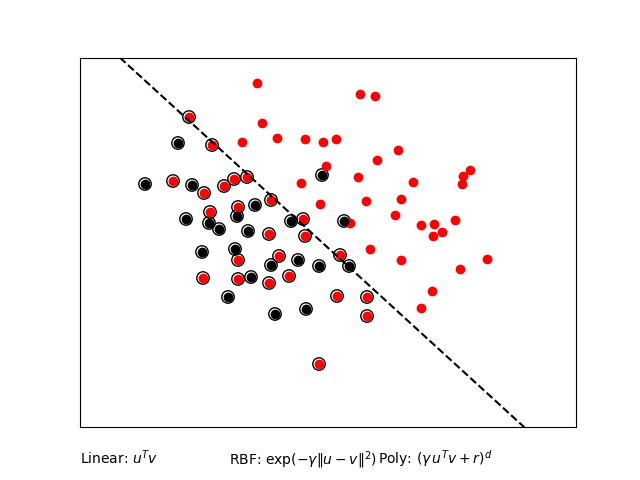
\includegraphics[width=\textwidth]{im000001.png}
        \caption{SVM avec C = 0.00001 }
    \end{minipage}
\end{figure}

Lorsque le paramètre de régularisation \( C \) est élevé (comme dans la première image avec \( C = 1 \)), le SVM impose une séparation stricte des classes, minimisant les erreurs de classification mais avec une marge plus étroite. En réduisant \( C \) (deuxième image avec \( C = 0.0019 \)), le modèle devient plus souple, augmentant la largeur de la marge au prix de plus d'erreurs, notamment pour les points proches de la frontière de décision. Avec un \( C \) très faible (troisième image, \( C = 0.00001 \)), le SVM se concentre principalement sur l'élargissement de la marge, entraînant une séparation moins précise avec de nombreux points mal classés, particulièrement ceux de la classe minoritaire. Cela montre qu'un \( C \) trop petit conduit à une généralisation excessive, sacrifiant la précision au profit d'une marge plus large.

\section{Classification de visages}
\subsection{Influence du Paramètre de Régularisation \( C \)
 sur la Prédiction}
\paragraph{Chargement et Préparation des Données\\}
Nous avons commencé par télécharger et charger l'ensemble de données LFW en utilisant la fonction \texttt{fetch\_lfw\_people} de Scikit-learn. Nous avons sélectionné deux individus dans l'ensemble de données, à savoir "Tony Blair" et "Colin Powell". Ensuite, nous avons filtré les images pour ne conserver que celles de ces deux personnes.

\begin{lstlisting}[language=Python, caption=Chargement des données et prétraitement]
lfw_people = fetch_lfw_people(min_faces_per_person=70, resize=0.4, color=True)
names = ['Tony Blair', 'Colin Powell']
idx0 = (lfw_people.target == target_names.index(names[0]))
idx1 = (lfw_people.target == target_names.index(names[1]))
images = np.r_[images[idx0], images[idx1]]
n_samples = images.shape[0]
y = np.r_[np.zeros(np.sum(idx0)), np.ones(np.sum(idx1))].astype(int)
plot_gallery(images, np.arange(12))
plt.show()
\end{lstlisting}

Nous avons ensuite extrait les étiquettes pour chaque classe (0 pour Tony Blair et 1 pour Colin Powell) et préparé les données pour l'entraînement et les tests.

\begin{figure}[H]
    \centering
    \begin{minipage}{0.9\textwidth}
        \centering
        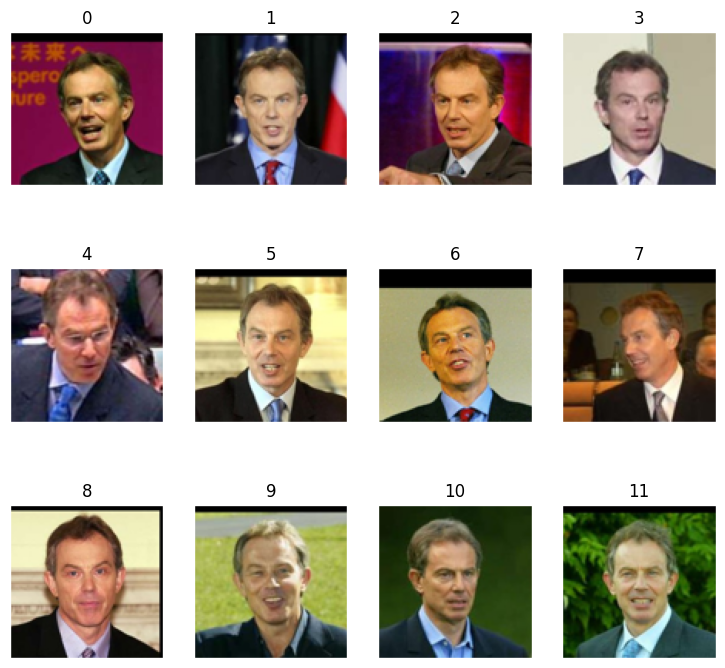
\includegraphics[width=\textwidth]{C11.png}
    \end{minipage}
    \end{figure}

\paragraph{Extraction des Caractéristiques\\}
Pour extraire les caractéristiques des images, nous avons choisi d'utiliser la moyenne des intensités des pixels en niveaux de gris pour chaque image. Chaque image a ensuite été redimensionnée en un vecteur plat.

\begin{lstlisting}[language=Python, caption=Extraction des caractéristiques]
X = (np.mean(images, axis=3)).reshape(n_samples, -1)
X -= np.mean(X, axis=0)
X /= np.std(X, axis=0)
\end{lstlisting}

\textbf{Explication :}
\begin{itemize}
    \item Normalisation des données : Chaque pixel est centré (moyenne = 0) et mis à l'échelle (écart-type = 1) afin de standardiser les données avant l'entraînement du modèle.
\end{itemize}

\paragraph{Séparation des Données d'Entraînement et de Test}
Les données ont été divisées en un ensemble d'entraînement (50\%) et un ensemble de test (50\%) à l'aide d'une permutation aléatoire. Cela permet de garantir que les résultats obtenus ne sont pas biaisés par une division spécifique des données.

\begin{lstlisting}[language=Python, caption=Séparation des données]
indices = np.random.permutation(X.shape[0])
train_idx, test_idx = indices[:X.shape[0] // 2], indices[X.shape[0] // 2:]
X_train, X_test = X[train_idx, :], X[test_idx, :]
\end{lstlisting}

\textbf{Résultat :}
\begin{itemize}
    \item Ensemble d'entraînement : 50\% des données.
    \item Ensemble de test : 50\% des données.
\end{itemize}

\paragraph{Ajustement du Modèle SVM avec Noyau Linéaire\\}
Nous avons entraîné plusieurs modèles SVM en utilisant un noyau linéaire avec différentes valeurs du paramètre de régularisation \( C \) (allant de \( 10^{-5} \) à \( 10^{5} \)). Le but était de déterminer la meilleure valeur de \( C \) en fonction de la précision sur l'ensemble de test.

\begin{lstlisting}[language=Python, caption=Ajustement du modèle SVM]
Cs = 10. ** np.arange(-5, 6)
scores = []
for C in Cs:
    clf = SVC(kernel='linear', C=C)
    clf.fit(X_train, y_train)
    y_pred = clf.predict(X_test)
    scores.append(accuracy_score(y_test, y_pred ))
\end{lstlisting}

Ensuite, nous avons identifié la meilleure valeur de \( C \) et affiché la courbe des scores en fonction de \( C \).

\begin{lstlisting}[language=Python, caption=Sélection de la meilleure valeur de C]
# Trouver la valeur de C qui donne le meilleur score
ind = np.argmax(scores)
print("Best C: {}".format(Cs[ind]))
# Afficher la courbe des scores en fonction de C
plt.figure()
plt.plot(Cs, scores)
plt.xlabel("Paramètres de régularisation C")
plt.ylabel("Scores d'apprentissage (accuracy)")
plt.xscale("log")
plt.tight_layout()
plt.show()
print("Best score: {}".format(np.max(scores)))
\end{lstlisting}

\begin{figure}[H]
    \centering
    \begin{minipage}{0.9\textwidth}
        \centering
        \includegraphics[width=\textwidth]{C2.png}
        \caption{ Impact du Paramètre de Régularisation 
 sur l'Accuracy }
    \end{minipage}
    \end{figure}
Les résultats indiquent que la meilleure régularisation est obtenue avec \(C = 0.001\), où le modèle atteint une précision de 93\%. Avec des valeurs très faibles de \(C\), la précision est d'environ 60\%, mais elle augmente rapidement jusqu'à \(C = 0.001\), avant de se stabiliser. Cela montre que cette valeur de \(C\) fournit le bon équilibre entre généralisation et performance pour cette tâche de reconnaissance de visages.

\paragraph{Prédiction des étiquettes des images de test\\}

Dans cette partie, nous utilisons le meilleur classificateur précédemment entraîné pour prédire les étiquettes des images de l'ensemble de test. Nous mesurons également le temps d'exécution et évaluons la précision du modèle. Le code utilisé est présenté ci-dessous.

\begin{lstlisting}[language=Python, caption=Prédiction des étiquettes des images de test avec le meilleur classificateur]
# predict labels for the X_test images with the best classifier
clf = best_clf
t0 = time()
y_pred = clf.predict(X_test)  # Prédiction des labels
print("done in %0.3fs" % (time() - t0))
print("Chance level : %s" % max(np.mean(y), 1. - np.mean(y)))
print("Accuracy : %s" % clf.score(X_test, y_test))  # Accuracy du meilleur modèle
\end{lstlisting}
\begin{itemize}
  \item Temps d'exécution : 0.281s
  \item Niveau de chance : 62.1\%
  \item Précision du modèle : 90\%
\end{itemize}

\paragraph{Évaluation qualitative des prédictions\\}
Nous avons généré des titres comparant la prédiction du modèle à la vérité terrain, et nous avons affiché une galerie d'images pour une évaluation visuelle des résultats.

\begin{lstlisting}[language=Python, caption=Évaluation des prédictions avec Matplotlib]
# Fonction pour générer des titres selon la prédiction et la vérité terrain
def title(pred, true, names):
    pred_name = names[int(pred)]
    true_name = names[int(true)]
    return f"Pred: {pred_name}\nTrue: {true_name}"
# Créer les titres basés sur les prédictions
prediction_titles = [title(y_pred[i], y_test[i], names) for i in range(y_pred.shape[0])]
# Afficher la galerie d'images avec les prédictions
plot_gallery(images_test, prediction_titles)
plt.show()
\end{lstlisting}
\begin{figure}[H]
    \centering
    \begin{minipage}{0.9\textwidth}
        \centering
        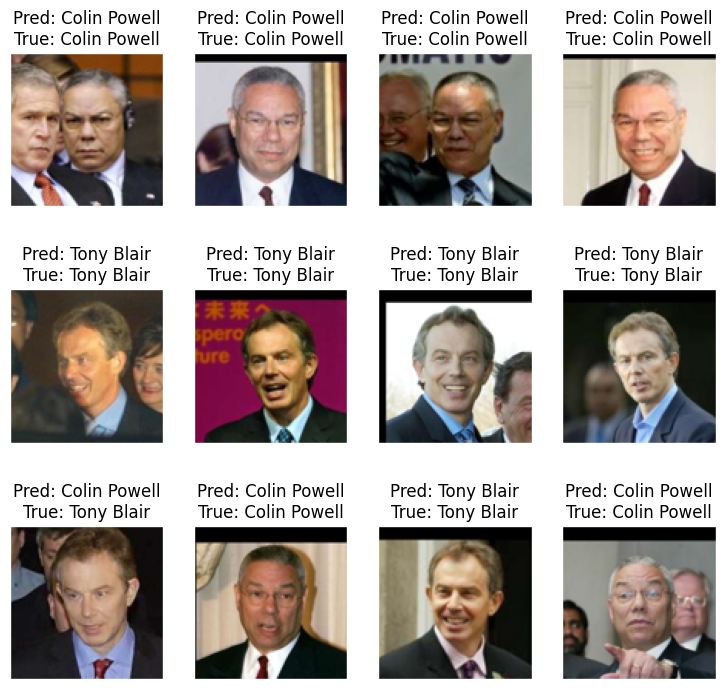
\includegraphics[width=\textwidth]{C3.png}
        \caption{ Classification des Visages }
    \end{minipage}
    \end{figure}
Le modèle parvient globalement à bien prédire les visages de Colin Powell et Tony Blair, mais montre quelques erreurs de classification. Ces erreurs peuvent être dues à la variabilité et la qualités des images ou à des limitations du modèle.    
\paragraph{Visualisation des coefficients pour un noyau linéaire\\}
 Nous avons affiché une carte de chaleur des coefficients si le modèle utilise un noyau linéaire. Cette carte montre l'importance de chaque pixel dans la prise de décision du modèle.

\begin{lstlisting}[language=Python, caption=Visualisation des coefficients du modèle linéaire]
# Afficher les coefficients sous forme d'image (pour un noyau linéaire)
if clf.kernel == 'linear':  # Ce plot fonctionne uniquement pour un noyau linéaire
    plt.figure()
    # Afficher les coefficients sous forme d'image (correspond à l'importance des pixels)
    plt.imshow(np.reshape(clf.coef_[0], (h, w)), interpolation='nearest', cmap=plt.cm.hot)
    plt.title("Coefficient image (importance des pixels)")
    plt.colorbar()
    plt.show()
else:
    print("Le modèle n'est pas linéaire, donc les coefficients ne peuvent pas être affichés.")
\end{lstlisting}
\begin{figure}[H]
    \centering
    \begin{minipage}{0.9\textwidth}
        \centering
        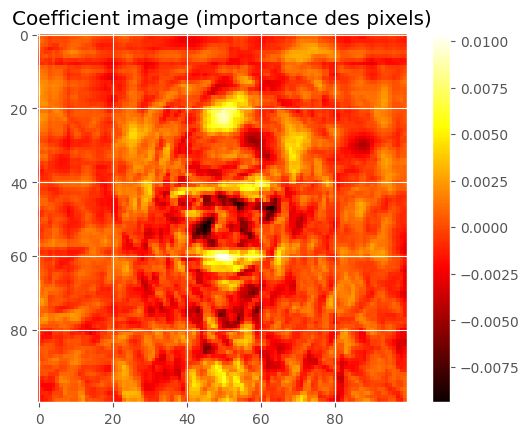
\includegraphics[width=\textwidth]{C4.png}
        \caption{ Importance des Pixels pour la Classification avec un SVM}
    \end{minipage}
    \end{figure}
L'image montre une carte de chaleur des coefficients du modèle SVM linéaire, indiquant les pixels les plus influents pour la classification. Les zones lumineuses (jaune) représentent les pixels clés dans la prise de décision, tandis que les zones sombres (en rouge ou noir) ont un impact moindre.

\subsection{Impact des Variables de Nuisance sur la Performance d'un Modèle SVM}
L'objectif de ce code est de démontrer que l'ajout de variables de nuisance (bruit) aux données d'apprentissage dégrade la performance du modèle SVM. Nous allons d'abord exécuter le modèle SVM sur les données d'origine, puis ajouter des variables de nuisance et comparer les performances sur l'ensemble de test.

\begin{lstlisting}
# Fonction pour entraîner et évaluer le modèle SVM linéaire
def run_svm_cv(_X, _y):
    # Permutation aléatoire des données
    _indices = np.random.permutation(_X.shape[0])
    _train_idx, _test_idx = _indices[:_X.shape[0] // 2], _indices[_X.shape[0] // 2:]
    # Séparation des données en ensembles d'entraînement et de test
    _X_train, _X_test = _X[_train_idx, :], _X[_test_idx, :]
    _y_train, _y_test = _y[_train_idx], _y[_test_idx]
    # Paramètres pour SVM linéaire (variation de C sur une plage logarithmique)
    _parameters = {'kernel': ['linear'], 'C': list(np.logspace(-3, 3, 5))}
    _svr = svm.SVC()
    _clf_linear = GridSearchCV(_svr, _parameters)   
    # Entraînement du modèle
    _clf_linear.fit(_X_train, _y_train)
    # Affichage des scores sur les ensembles d'entraînement et de test
    print('Generalization score for linear kernel: %s, %s \n' %
          (_clf_linear.score(_X_train, _y_train), _clf_linear.score(_X_test, _y_test)))
# Exécution du modèle SVM sur les données sans nuisance
print("Score sans variable de nuisance")
run_svm_cv(X, y)
\end{lstlisting}
\begin{lstlisting}
# Ajout de variables de nuisance (bruit gaussien)
n_features = X.shape[1]
sigma = 1
noise = sigma * np.random.randn(n_samples, 300)
# Concaténation du bruit avec les données d'origine
X_noisy = np.concatenate((X, noise), axis=1)
X_noisy = X_noisy[np.random.permutation(X.shape[0])]  # Permutation aléatoire
# Exécution du modèle SVM sur les données avec variables de nuisance
print("Score avec variables de nuisance")
run_svm_cv(X_noisy, y)
\end{lstlisting}
\begin{figure}[H]
    \centering
    \begin{minipage}{0.9\textwidth}
        \centering
        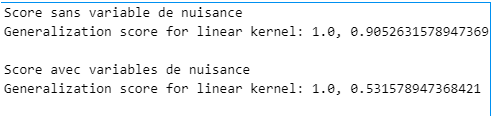
\includegraphics[width=\textwidth]{C12.PNG}
       
    \end{minipage}
    \end{figure}
L'ajout de variables de nuisance aux données a un impact négatif important sur la performance du modèle SVM. Les variables de nuisance augmentent la dimension des données sans ajouter d'information utile, ce qui entraîne une baisse significative de la capacité du modèle à généraliser sur des données qu'il n'a pas vues.
\subsection{Amélioration des Prédictions avec Réduction de Dimension par PCA}

Nous avons appliqué une réduction de dimension avec PCA sur des données bruitées, en utilisant un nombre ajustable de composantes principales. Nous avons fixé initialement le paramètre à 20 et affiché la variance expliquée pour vérifier si ces composantes capturent une quantité suffisante d'information dans les données.

\begin{lstlisting}[language=Python, caption=Application de PCA avec affichage de la variance expliquée]
# Application de la PCA sur les données bruitées
n_components = 20  # Nombre de CP (peut être ajusté)
pca = PCA(n_components=n_components, svd_solver='randomized').fit(X_noisy)
# Transformation des données avec PCA
X_noisy_pca = pca.transform(X_noisy)
explained_variance = np.sum(pca.explained_variance_ratio_)
print(f"Variance expliquée avec {n_components} composantes : {explained_variance:.2%}")
\end{lstlisting}
Avec 20 composantes principales, la réduction de dimension capture 67.68 \% de la variance totale, conservant ainsi une bonne partie de l'information tout en réduisant la complexité. En revanche, avec seulement 3 composantes, seulement 35.35 \% de la variance est expliquée, ce qui entraîne une perte significative d'information. Enfin, en augmentant à 30 composantes, la variance expliquée atteint 73.57 \%, ce qui montre une légère amélioration par rapport aux 20 composantes, mais avec un gain modéré.


\section*{Conclusion générale}

Les \textbf{SVM} sont des outils de classification puissants, capables de traiter des données complexes grâce à des noyaux adaptés. Cependant, leur performance dépend fortement de la sélection des paramètres, comme \( C \) et le choix du noyau, ainsi que de la qualité des données. Les techniques de réduction de dimension, telles que \textbf{PCA}, sont également cruciales pour améliorer la capacité du modèle à généraliser, surtout lorsque des variables de nuisance sont présentes.

Ce TP a permis d'acquérir une compréhension pratique de l'importance du réglage des hyperparamètres et de la gestion des données bruitées dans l'application des SVM à des problèmes de classification réels.

\end{document}


